\documentclass{article}
% Useful packages
\usepackage{amsmath}
\usepackage{graphicx}
\usepackage{amssymb}
\usepackage[colorlinks=true, allcolors=blue]{hyperref}

\title{Problem Set 3 Econometrics}
\author{Tai Wu}
\date{24/11/2024}
\begin{document}
\maketitle

\section*{}

\begin{figure}[!htbp]
    \centering
    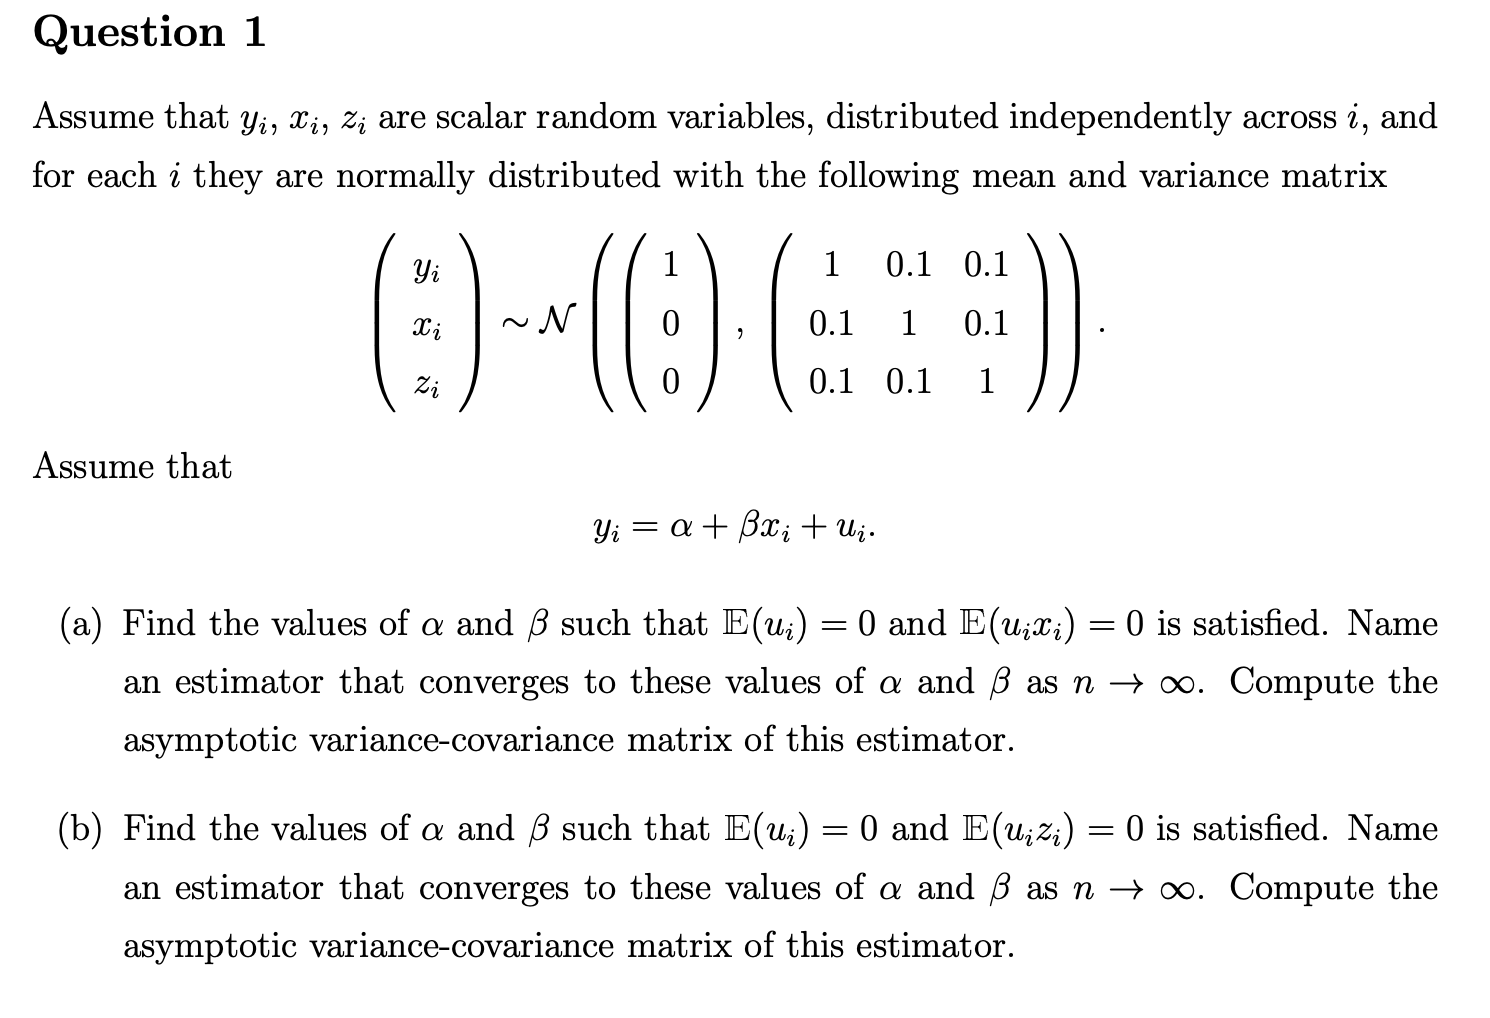
\includegraphics[width=1\linewidth]{question 1.png}
\end{figure}

\subsection*{Ans 1.a }
From \( \mathbb{E}(u_i)  = 0\) we have
\begin{align*}
\mathbb{E}(u_i) &= \mathbb{E}(y_i - \alpha - \beta x_i) \\
                &= \mathbb{E}(y_i) - \alpha - \beta \mathbb{E}(x_i) \\
                &= 1 - \alpha - 0 = 0 \\
\therefore \quad &\alpha = 1.
\end{align*}

From \( \mathbb{E}(u_i x_i) =0\) we have:
\begin{align*}
\mathbb{E}(u_i x_i) &= \mathbb{E}((y_i - \alpha - \beta x_i) x_i) \quad \text{-- plug in } \alpha = 1 \\
                    &= \mathbb{E}((y_i x_i - x_i - \beta x_i^2)) \\
                    &= \mathbb{E}(y_i x_i) - \mathbb{E}(x_i) - \beta \mathbb{E}(x_i^2) \\
                    &= \mathbb{E}(y_i x_i) - 0 - \beta (\text{Var}(x_i) + \mathbb{E}(x_i)^2) \\
                    &= 0 + 0.1 - \beta = 0 \\
\therefore \quad &\beta = 0.1.
\end{align*}

Thus \( \alpha = 1, \beta = 0.1 \).

We can have OLS estimator converge to this value as \( n \to \infty \). Let \( \mathbf{X} \) be \( \begin{bmatrix} 1 & x_i \end{bmatrix} \). Then:
\begin{align*}
\hat{\beta}_{\text{OLS}} &= (\mathbf{X}' \mathbf{X})^{-1} \mathbf{X}' \mathbf{y} \\
                         &= (\mathbf{X}' \mathbf{X})^{-1} \mathbf{X}' \mathbf{y} -->_p \mathbb{E}(\mathbf{X}' \mathbf{X})^{-1} \mathbb{E}(\mathbf{X}' \mathbf{y}) \\
                         &= \begin{bmatrix} 1 & 0 \\ 0 & 1 \end{bmatrix}^{-1} \begin{bmatrix} 1 \\ 0.1 \end{bmatrix} \\
                         &= \begin{bmatrix} 1 \\ 0.1 \end{bmatrix} = \begin{bmatrix} \hat{\alpha} \\ \hat{\beta} \end{bmatrix}. 
\end{align*}

Given the homoscedasticity error, we have the asymptotic variance:
\begin{align*}
\text{Var}(\hat{\beta}_{\text{OLS}}) &= \sigma^2 (\mathbf{X}' \mathbf{X})^{-1} = \sigma^2 \begin{bmatrix} 1 & 0 \\ 0 & 1 \end{bmatrix}^{-1} = \sigma^2 \begin{bmatrix} 1 & 0 \\ 0 & 1 \end{bmatrix}.
\end{align*}

\subsection*{Ans 1.b}
Given that \( \mathbb{E}(u_i) = 0 \) we have:
\begin{align*}
\mathbb{E}(u_i) &= \mathbb{E}(y_i - \alpha - \beta x_i) \\
                &= \mathbb{E}(y_i) - \alpha - \beta \mathbb{E}(x_i) \\
                &= 1 - \alpha - 0 = 0  \\
\therefore \quad &\alpha = 1.
\end{align*}

From  \( \mathbb{E}(u_i x_i) = 0 \),  we have:
\begin{align*}
\mathbb{E}(u_i x_i) &= \mathbb{E}((y_i - \alpha - \beta x_i) x_i) \quad \text{--- plug in } \alpha = 1 \\
                    &= \mathbb{E}(y_i x_i) - \mathbb{E}(x_i) - \beta \mathbb{E}(x_i^2) \\
                    &= \text{Cov}(y_i, x_i) - 0 - \beta \text{Cov}(x_i, x_i) \\
                    &= 0.1 - \beta \cdot 0.1 = 0 \\
\therefore \quad &\beta = 1.
\end{align*}
For a instrumental variable estimator \( \hat{\beta}_{IV} \), we rewrite the variable with a constant term that \( z_i = (1, z_i) \) and \( x_i = (1, x_i) \), we have:
\begin{align*}
\hat{\beta}_{IV} &= (X'Z)^{-1} Z'y -->_p \mathbb{E}(\mathbf{Z}' \mathbf{X})^{-1} \mathbb{E}(\mathbf{Z}' \mathbf{y}) \\
                 &=  \begin{bmatrix} 1 & 0 \\ 0 & 0.1 \end{bmatrix}^{-1} \begin{bmatrix} 1 \\ 0.1 \end{bmatrix} \\
                 &= \begin{bmatrix}
                     1 \\ 1
                 \end{bmatrix} = \begin{bmatrix} \hat{\alpha} \\ \hat{\beta} \end{bmatrix}. 
\end{align*}

The asymptotic variance under homoscedasticity is given by:
\begin{align*}
\hat{\beta}_{IV} &\sim N(\beta, \frac{1}{n}\Sigma_{\hat{\beta}_{IV}})\\
\Sigma_{\hat{\beta}_{IV}} &= \mathbb{E}[(Z'X)]^{-1} \mathbb{E}[u_i^2 Z_i Z_i] \mathbb{E}[(Z'X)]^{-1}  \\
&= \frac{1}{0.1} \begin{pmatrix}
0.1 & 0\\
0 & 1
\end{pmatrix} 
\sigma^2 \begin{pmatrix}
1 & 0\\
0 & 1
\end{pmatrix} \frac{1}{0.1} \begin{pmatrix}
0.1 & 0\\
0 & 1
\end{pmatrix} \\
&= 100 \sigma^2 \begin{pmatrix}
0.01 & 0\\
0 & 1
\end{pmatrix}\\
&= \begin{pmatrix}
1 & 0\\
0 & 100
\end{pmatrix}
\end{align*}


\section*{Question 2}
\begin{figure}[!htbp]
    \centering
    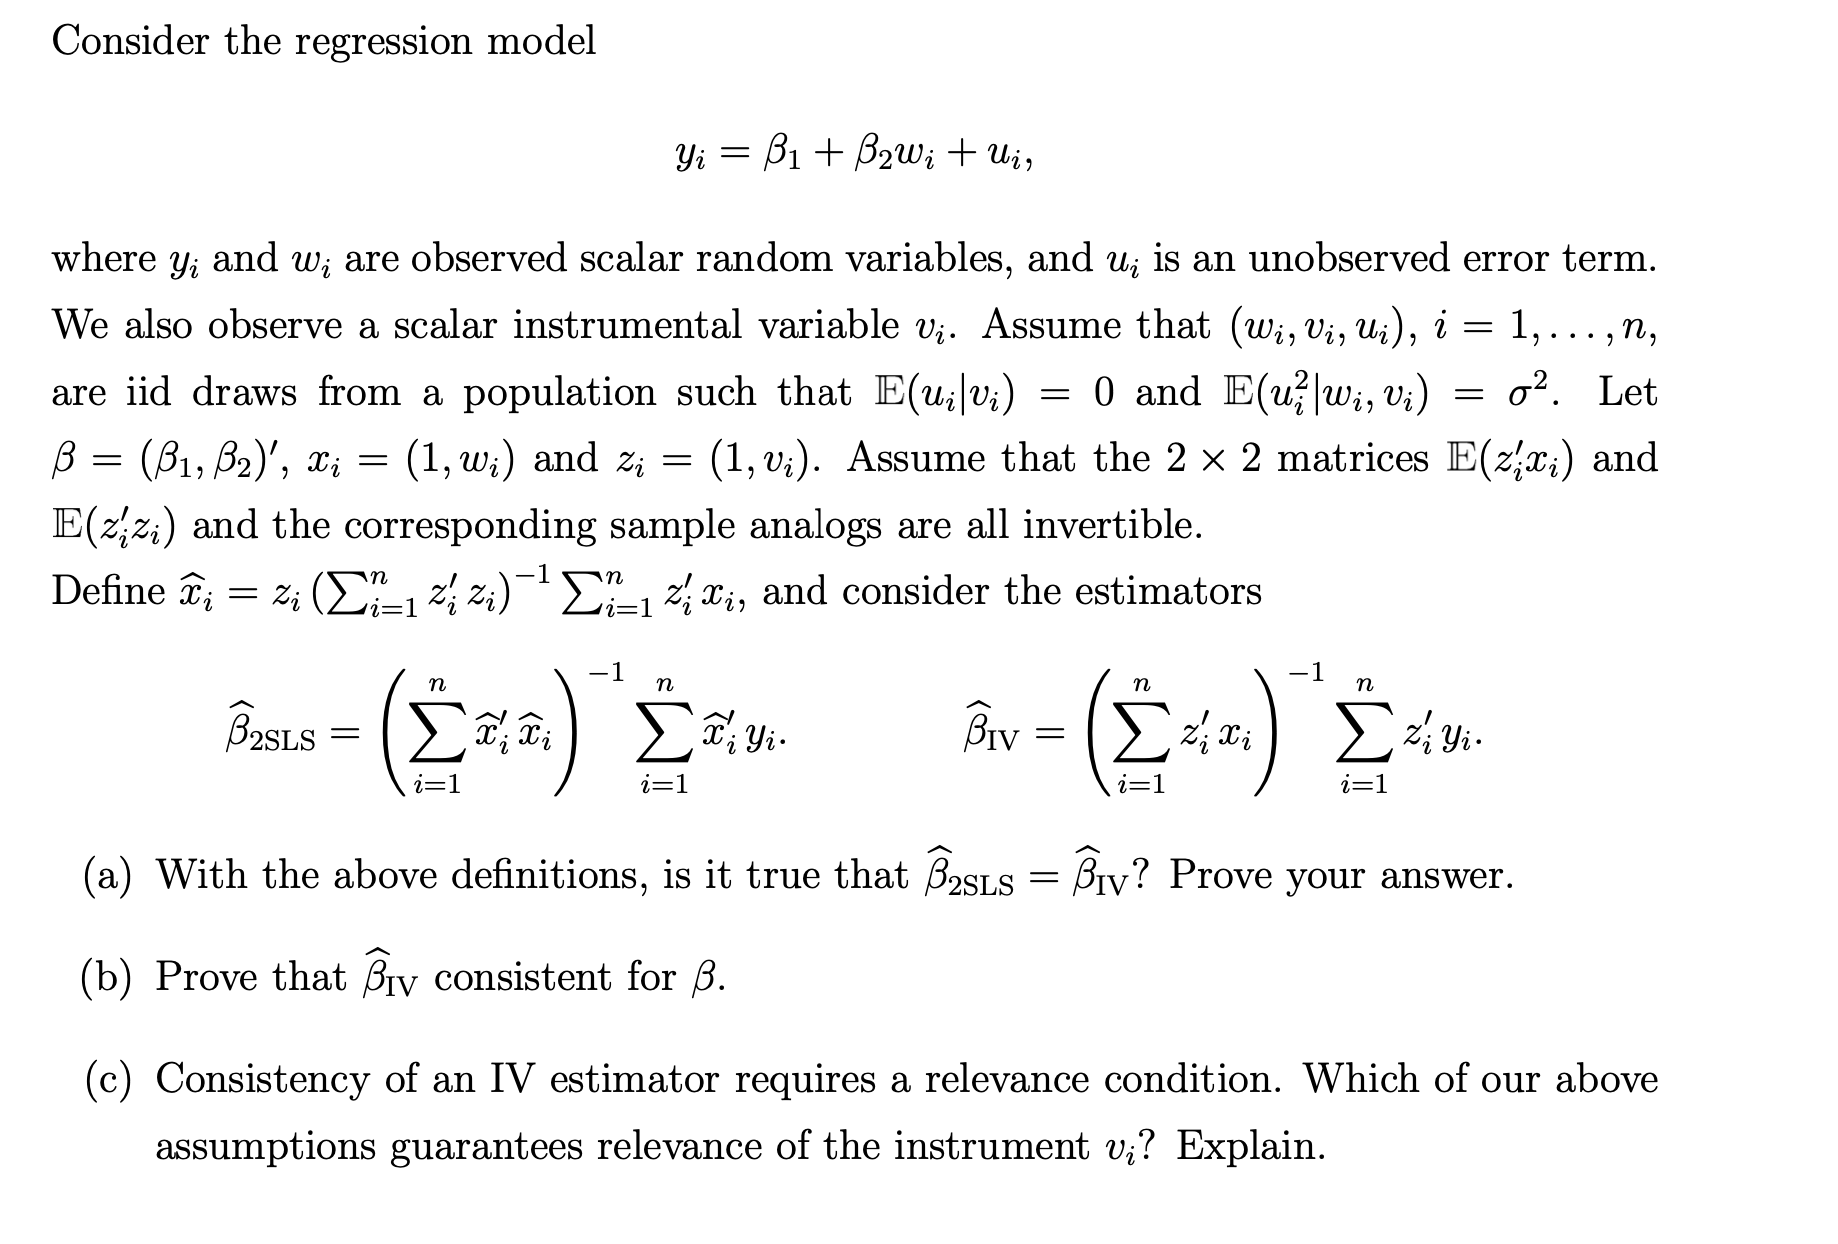
\includegraphics[width=1\linewidth]{Question 2.png}
\end{figure}
\subsection*{Ans 2.a }
Yes, with the above definition \( \hat{\beta}_{2SLS} = \hat{\beta}_{IV} \), we write in reduced matrix format:

Given $ \hat{X} = Z(Z'Z)^{-1}Z'X = P_Z X, \text{where } P_Z = Z(Z'Z)^{-1}Z'$ \\
\text{$P_Z$ is projector on $Z$ space, also $P_Z$ is symmetric and idempotent.}\\
\begin{align*}
\hat{\beta}_{2SLS} &= (X'X)^{-1}X'y \\
&= ((P_Z X)'P_Z X)^{-1}(P_Z X)'y \\
&= (X'P_Z X)^{-1}X'P_Z y \\
&= (X'Z(Z'Z)^{-1}Z'X)^{-1}X'Z(Z'Z)^{-1}Z'y \\
&= (Z'X)^{-1}(Z'Z)(X'Z)^{-1}X'Z(Z'Z)^{-1}Z'y \\
&= (Z'X)^{-1}Z'y = \left( \sum_{i=1}^{n} Z'_i X_i \right)^{-1} \left( \sum_{i=1}^{n} Z'_i y_i \right)= \hat{\beta}_{IV}.
\end{align*}


\subsection*{Ans 2.b }

To prove that \( \hat{\beta}_{IV} \) is consistent:
\begin{align*}
\hat{\beta}_{IV} &= \left( \sum_{i=1}^{n} Z'_i X_i \right)^{-1} \left( \sum_{i=1}^{n} Z'_i y_i \right)\\
&= \left( \frac{1}{n} \sum_{i=1}^{n} Z'_i X_i \right)^{-1} \frac{1}{n} \sum_{i=1}^{n} Z'_i X_i \beta + \left( \frac{1}{n} \sum_{i=1}^{n} Z'_i X_i \right)^{-1} \frac{1}{n} \sum_{i=1}^{n} Z'_i u_i\\
&= \beta + \left( \frac{1}{n} \sum_{i=1}^{n} Z'_i X_i \right)^{-1} \frac{1}{n} \sum_{i=1}^{n} Z'_i u_i
\end{align*}
By the Weak Law of Large Numbers (WLLN) it converges to: 
\[
\beta + \mathbb{E}(Z'X)^{-1} \mathbb{E}(Z'u) = \beta + \mathbb{E}(Z'X)^{-1} \begin{pmatrix} \mathbb{E}(u_i) \\ \mathbb{E}(v_i u_i) \end{pmatrix}
\]

By iterated expectation, given \(\mathbb{E}(u_i|v_i) = 0\) we have:
\begin{align*}
\mathbb{E}(u_i) &= \mathbb{E}(\mathbb{E}(u_i|v_i)) = 0, \\
\mathbb{E}(u_i v_i) &= \mathbb{E}(\mathbb{E}(u_i v_i|v_i)) = \mathbb{E}(v_i \mathbb{E}(u_i|v_i)) = \mathbb{E}(v_i \cdot 0) = 0.
\end{align*}


Therefore, \( \hat{\beta}_{IV} \) is a consistent estimator of \( \beta \).

\subsection*{Ans 2.c }
From \( \hat{\beta}_{IV} = \left( \sum_{i=1}^{n} Z_i'X_i \right)^{-1} \left( \sum_{i=1}^{n} Z_i'y_i \right) \), the relevance condition is from \( \mathbb{E}(Z_i'X_i) \) being invertible.

Meanwhile, the well-defined IV estimator also require \( \mathbb{E}(Z_i'Z_i) \) being invertible.

\section*{Question 3}
\begin{figure}[!htbp]
    \centering
    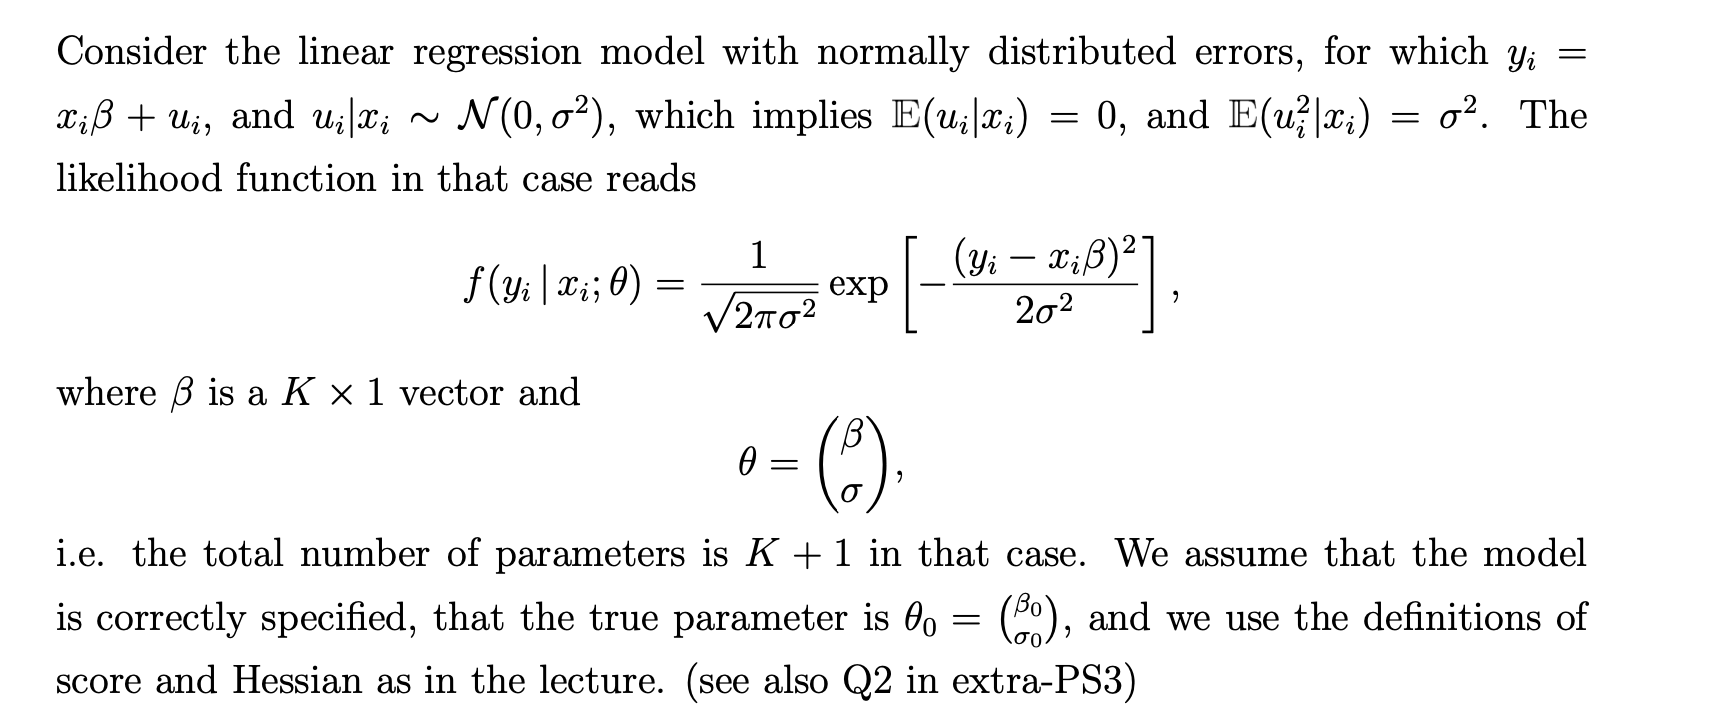
\includegraphics[width=1\linewidth]{question 3.png}
\end{figure}

\subsection*{Ans 3.a } Calculate the score \( s(y_i, x_i, \theta) \) and the Hessian \( H(y_i, x_i, \theta) \) for this model.

Given the likelihood function
\[
f(y_i | x_i; \theta) = \frac{1}{\sqrt{2\pi\sigma^2}} \exp \left( -\frac{(y_i - x_i\beta)^2}{2\sigma^2} \right), \quad \theta = \begin{pmatrix} \beta \\ \sigma \end{pmatrix}.
\]

The log-likelihood \(\ell(\theta)\) is:
\[
\ell(\theta) = -\frac{1}{2}\log(2\pi) - \frac{1}{2}\log(\sigma^2) - \frac{1}{2\sigma^2}(y_i - x_i\beta)^2.
\]

The score \(s(y_i, x_i; \theta)\) is:
\[
s(y_i, x_i; \theta) = \begin{pmatrix}
\frac{\partial \ell(\theta)}{\partial \beta} \\
\frac{\partial \ell(\theta)}{\partial \sigma}
\end{pmatrix}.
\]

Where:
\[
\frac{\partial \ell(\theta)}{\partial \beta} = \frac{1}{\sigma^2} x_i(y_i - x_i\beta),
\]

\[
\frac{\partial \ell(\theta)}{\partial \sigma} = -\frac{1}{\sigma} + \frac{1}{\sigma^3} (y_i - x_i\beta)^2.
\]

Thus, the score and Hessian is given by:
\[
s(y_i | x_i; \theta) = \begin{pmatrix}
\frac{1}{\sigma^2} x_i(y_i - x_i\beta) \\
-\frac{1}{\sigma} + \frac{1}{\sigma^3} (y_i - x_i\beta)^2
\end{pmatrix},  \quad H =\begin{pmatrix}
-\frac{1}{\sigma^2} x_i\cdot x_i & -\frac{2}{\sigma^3}x_i(y_i - x_i\beta) \\
-\frac{2}{\sigma^3}x_i(y_i - x_i\beta) & -\frac{1}{2\sigma^2} + \frac{3}{\sigma^4}(y_i - x_i\beta)^2
\end{pmatrix}.
\]

\subsection*{Ans 3.b } Show that

To show $\mathbb{E}\left[s\left(y_i, x_i, \theta_0\right)\left(x_i\right]=0\right.$
$$
\mathbb{E}\left[\frac{1}{\sigma_0^2} x_i\left(y_i-x_i \beta\right) \mid x_i\right]=\frac{x_i}{\sigma_0^2} \mathbb{E}\left[y_i-x_i\beta \mid x_i\right]= \frac{x_i}{\sigma_0^2} \mathbb{E}\left[u_i \mid x_i\right]=0
$$
Since by normality assumption, $\mathbb{E}\left[u_i \mid x_i\right]=0$


$$
\begin{aligned}
\mathbb{E}\left(-\frac{1}{\sigma_0}+\left(y_i-x_i \beta\right)^2 \cdot \frac{1}{\sigma_0^3} \mid x_i\right)=\mathbb{E}\left[-\frac{1}{\sigma_0}+u_i^2 \cdot \frac{1}{\sigma_0^3} \mid x_i\right] & =\mathbb{E}\left(-\frac{1}{\sigma_0}\right)+\frac{1}{\sigma_0^3} \mathbb{E}\left(u_i^2 \mid x_i\right) \\
\text { Since } \sigma_0 \text { is true parameter, } \sigma_0=\sigma \quad & =-\frac{1}{\sigma_0}+\frac{1}{\sigma_0}=0
\end{aligned}
$$

$\begin{aligned} & \text { Therefore } \\ & \qquad\left(s\left(y_i, x_i, \theta_0\right) \mid x_i\right)=\left(\begin{array}{l}\mathbb{E}\left(\frac{1}{\sigma_0^2} x_i\left(y_i-x_i \beta\right) \mid x_i\right. \\ \mathbb{E}\left(-\frac{1}{\sigma_0}+u_i^2 \cdot \frac{1}{\sigma_0^3} \mid x_i\right.\end{array}\right)=\left(\begin{array}{l}0 \\ 0\end{array}\right)\end{aligned}$

\subsection*{Ans 3.c }
Find $\mathbb{E}\left[H\left(y_i, x_i, \theta_0\right)\right]$
$H\left(y_i, x_i, \theta_0 \right)$ is given by
$$
\begin{aligned}
H & =\left(\begin{array}{cc}
-\frac{1}{\sigma^2} x_i \cdot x_i & -\frac{2}{\sigma^3} x_i\left(y_i-x_i \beta\right) \\
-\frac{2}{\sigma^3} x_i\left(y_i-x_i \beta\right) & \frac{1}{\sigma^2}-\frac{3}{\sigma^4}\left(y_i-x_i \beta\right)^2
\end{array}\right)
\end{aligned}\\
$$

$$
\begin{aligned}
E\left(H\left(y_i, x_i, \theta_0\right)\right) & =\left(\begin{array}{cc}
-\frac{1}{\sigma_0^2} \mathbb{E}\left(x_i x_i\right) & -2 \cdot \frac{1}{\sigma^3} \mathbb{E}\left(x_i u_i\right) \\
-2 \frac{1}{\sigma_0^3} \mathbb{E}\left(x_i u_i\right) & \frac{1}{\sigma_0^2}-\frac{3}{\sigma_0^4} \mathbb{E}\left(u_i^2\right)
\end{array}\right) \\
& =\left(\begin{array}{cc}
-\frac{1}{\sigma_0^2} \mathbb{E}\left(x_i x_i\right) & 0 \\
0 & -\frac{2}{\sigma_0^2}
\end{array}\right)
\end{aligned}
$$
\subsection*{Ans 3.d }Assume that $\sigma_0^2>0$. Provide a non-collinearity condition on the regressors $x_i$ that guarantees that $\mathbb{E}\left[H\left(y_i, x_i, \theta_0\right)\right]$ is invertible.

Ans: we have $\left[-E\left(H\left(y_i, x_i, \theta_0\right)\right)\right]^{-1}=\left(\begin{array}{cc}\sigma_0^2 E\left(x_i x_i\right)^{-1} & 0 \\ 0 & \frac{\sigma_0^2}{2}\end{array}\right)$. The non-collinearity condition on the regressor is given by $E\left(x_i x_i\right)^{-1}$ is invertible thant is the $\operatorname{rank}\left(E\left(x_i x_i\right)\right)=k$.

\subsection*{Ans 3.e }
Calculate the asymptotic variance covariance matrix $\Sigma_\theta$, which satisfies $\sqrt{n}(\hat{\theta}-$ $\left.\theta_0\right) \Rightarrow \mathcal{N}\left(0, \Sigma_\theta\right)$.

Ans: $\text{We have } \hat{\theta}_{\text{MLE}} = \operatorname{arg}_{\theta \in(\Theta)} \max \log f\left(y_i, x_i ; 0\right) \\ $

$\begin{aligned} 
\sqrt{n}(\hat{\theta} - \theta_0) \Rightarrow & N(0, \Sigma_\theta) \\ 
& \Sigma_\theta = \mathcal{I}^{-1} = \left\{\operatorname{Var}\left(s (y_i, x_i, \theta_0\right)\right\}^{-1} = \left\{-E\left[H\left(y_i, x_i, \theta_0\right)\right]\right\}^{-1} \\ 
& = \left(\begin{array}{cc} \sigma_0^2 \mathbb{E}(X_i' X_i)^{-1} & 0 \\ 0 & \frac{\sigma_0^2}{2} \end{array}\right) = \Sigma_\theta
\end{aligned}$


\end{document}